\section{Theoretical Analysis}
\label{sec:theory}

We develop a formal framework to explain why per-class adaptive guidance outperforms fixed guidance, why cluster entropy and intra-class variance are the effective complexity factors, and why inter-class separability is not. Our analysis proceeds under a Gaussian mixture model for the class-conditional distribution, which is the standard approximation for multi-modal class structure in feature space~\cite{ho2022classifierfree, peebles2022scalable}.

\paragraph{Setup.}
Consider a class $c$ whose conditional distribution is a $K_c$-component Gaussian mixture:
\begin{equation}
p(\mathbf{x} \mid c) = \sum_{k=1}^{K_c} \pi_{c,k}\,\mathcal{N}(\mathbf{x};\,\boldsymbol{\mu}_{c,k},\,\boldsymbol{\Sigma}_{c,k}),
\label{eq:gmm}
\end{equation}
where $\pi_{c,k} > 0$ are mode proportions satisfying $\sum_k \pi_{c,k} = 1$. The cluster entropy $H_c = -\sum_k \pi_{c,k}\log\pi_{c,k}$ measures the balance of mode sizes, and the intra-class variance $v_c = \mathrm{tr}[\bar{\boldsymbol{\Sigma}}_c] = \mathrm{tr}\!\left[\sum_k \pi_{c,k}\,\boldsymbol{\Sigma}_{c,k}\right]$ measures the total feature spread. Under CFG with scale $\lambda$ (Eq.~\eqref{eq:cfg}), the effective conditional distribution is $p_\lambda(\mathbf{x}\mid c) \propto p(\mathbf{x}\mid c)^{1+\lambda}\,p(\mathbf{x})^{-\lambda}$.

\begin{lemma}[CFG Mode Sharpening and Reweighting]
\label{lem:cfg-modes}
For well-separated modes (i.e., $\|\boldsymbol{\mu}_{c,j} - \boldsymbol{\mu}_{c,k}\| \gg \mathrm{tr}[\boldsymbol{\Sigma}_{c,k}]$ for $j \neq k$), the CFG-modified distribution is approximately
\begin{equation}
p_\lambda(\mathbf{x}\mid c) \approx \sum_{k=1}^{K_c} \tilde{\pi}_{c,k}(\lambda)\,\mathcal{N}\!\left(\mathbf{x};\,\boldsymbol{\mu}_{c,k},\,\tfrac{\boldsymbol{\Sigma}_{c,k}}{1+\lambda}\right),
\label{eq:cfg-gmm}
\end{equation}
where the effective mode weights are $\tilde{\pi}_{c,k}(\lambda) = \pi_{c,k}^{1+\lambda}\big/\sum_j \pi_{c,j}^{1+\lambda}$. Thus CFG has two effects: (i) \emph{sharpening}---each mode's covariance is scaled by $1/(1+\lambda)$---and (ii) \emph{reweighting}---dominant modes (large $\pi_{c,k}$) receive proportionally more weight.
\end{lemma}

\begin{proof}
For well-separated modes, $p(\mathbf{x}\mid c)^{1+\lambda} \approx \sum_k \pi_{c,k}^{1+\lambda}\,\mathcal{N}(\mathbf{x};\boldsymbol{\mu}_{c,k},\boldsymbol{\Sigma}_{c,k})^{1+\lambda}$ in each mode's support. Since $\mathcal{N}(\mathbf{x};\boldsymbol{\mu},\boldsymbol{\Sigma})^{1+\lambda} \propto \mathcal{N}(\mathbf{x};\boldsymbol{\mu},\boldsymbol{\Sigma}/(1+\lambda))$ (a Gaussian raised to a power remains Gaussian with rescaled covariance), the result follows. The $p(\mathbf{x})^{-\lambda}$ term contributes a slowly-varying factor that we absorb into the normalization; this is exact when $p(\mathbf{x})$ is uniform and approximate otherwise.
\end{proof}

\begin{proposition}[Diversity Cost of Guidance]
\label{prop:div-cost}
The Kullback--Leibler divergence between the original and reweighted mode distributions,
\begin{equation}
D_c(\lambda) := \mathrm{KL}\!\left(\boldsymbol{\pi}_c \,\|\, \tilde{\boldsymbol{\pi}}_c(\lambda)\right) = \lambda\,H_c + \log Z_c(\lambda),
\label{eq:div-cost}
\end{equation}
where $Z_c(\lambda) = \sum_k \pi_{c,k}^{1+\lambda}$, satisfies:
\begin{enumerate}
    \item[(a)] $D_c(0) = 0$ and $D_c'(0) = 0$ (no first-order diversity loss at $\lambda = 0$);
    \item[(b)] $D_c''(0) = \mathrm{Var}_{\boldsymbol{\pi}_c}[\log\pi_{c,k}]$, the variance of log-mode-probabilities;
    \item[(c)] $D_c''(0)$ is \emph{decreasing in} $H_c$: balanced (high-entropy) classes incur lower diversity cost.
\end{enumerate}
\end{proposition}

\begin{proof}
Substituting $\tilde{\pi}_k = \pi_k^{1+\lambda}/Z$ into the KL divergence yields $D_c(\lambda) = \sum_k \pi_k \log\pi_k - \sum_k \pi_k[(1{+}\lambda)\log\pi_k - \log Z] = \lambda H_c + \log Z$. For (a), $Z(0) = 1$ and $Z'(0) = \sum_k \pi_k \log\pi_k = -H_c$, so $D_c'(0) = H_c + Z'(0)/Z(0) = 0$. For (b), $Z''(0) = \sum_k \pi_k(\log\pi_k)^2$, giving $D_c''(0) = Z''(0) - Z'(0)^2 = \sum_k \pi_k(\log\pi_k)^2 - H_c^2 = \mathrm{Var}_{\boldsymbol{\pi}_c}[\log\pi_k]$. For (c), $\mathrm{Var}[\log\pi_k] = \mathbb{E}[(\log\pi_k)^2] - (\mathbb{E}[\log\pi_k])^2 = \mathbb{E}[(\log\pi_k)^2] - H_c^2$. Since $\log$ is concave, $\mathbb{E}[(\log\pi_k)^2]$ is Schur-convex and $H_c$ is Schur-concave; as the distribution becomes more balanced ($H_c$ increases), both terms converge, driving the variance to zero at maximum entropy (all $\pi_k = 1/K_c$).
\end{proof}

Proposition~\ref{prop:div-cost} establishes that the diversity cost of guidance is governed by the \emph{logit variance} $\sigma_c^2 := \mathrm{Var}_{\boldsymbol{\pi}_c}[\log\pi_{c,k}]$, not by entropy directly. High-entropy classes (balanced modes) have $\sigma_c^2 \approx 0$ and incur negligible diversity cost, while low-entropy classes (dominant mode) have large $\sigma_c^2$ and lose minor modes rapidly.

\begin{proposition}[Optimal Per-Class Guidance]
\label{prop:opt-lambda}
Define the per-class generation utility under guidance $\lambda$ as
\begin{equation}
U_c(\lambda) = (1+\lambda)\,v_c - \beta\,D_c(\lambda),
\label{eq:utility}
\end{equation}
where $v_c$ is the intra-class variance, $\beta > 0$ is a trade-off parameter, and $D_c(\lambda)$ is the diversity cost (Proposition~\ref{prop:div-cost}). The optimal guidance $\lambda_c^* = \arg\max_\lambda U_c(\lambda)$ satisfies, to second order:
\begin{equation}
\lambda_c^* \approx \frac{v_c}{\beta\,\sigma_c^2},
\label{eq:opt-lambda}
\end{equation}
where $\sigma_c^2 = \mathrm{Var}_{\boldsymbol{\pi}_c}[\log\pi_{c,k}]$. Consequently, $\lambda_c^*$ is \emph{increasing in} $v_c$ (intra-class variance) and \emph{increasing in} $H_c$ (cluster entropy, since $\sigma_c^2$ is decreasing in $H_c$).
\end{proposition}

\begin{proof}
By Proposition~\ref{prop:div-cost}, $D_c(\lambda) \approx \frac{1}{2}\sigma_c^2\,\lambda^2$ for small $\lambda$ (using $D_c(0) = D_c'(0) = 0$ and $D_c''(0) = \sigma_c^2$). Substituting into Eq.~\eqref{eq:utility}: $U_c(\lambda) \approx v_c + v_c\lambda - \frac{\beta}{2}\sigma_c^2\,\lambda^2$. Setting $U_c'(\lambda) = v_c - \beta\,\sigma_c^2\,\lambda = 0$ yields $\lambda_c^* = v_c / (\beta\,\sigma_c^2)$. The monotonicity claims follow: $\partial\lambda_c^*/\partial v_c = 1/(\beta\,\sigma_c^2) > 0$, and $\partial\lambda_c^*/\partial H_c = -v_c/(\beta\,\sigma_c^4)\cdot\partial\sigma_c^2/\partial H_c > 0$ since $\partial\sigma_c^2/\partial H_c < 0$ by Proposition~\ref{prop:div-cost}(c).
\end{proof}

Proposition~\ref{prop:opt-lambda} provides the central theoretical insight: the optimal guidance strength for class $c$ is determined by the ratio of its intra-class variance $v_c$ (the benefit of sharpening) to its logit variance $\sigma_c^2$ (the cost of reweighting). Since $\sigma_c^2$ decreases with entropy $H_c$, high-entropy classes can sustain stronger guidance. This explains why CAGS assigns higher $\lambda$ to classes with high entropy and high intra-class variance.

\begin{theorem}[Adaptivity Gap]
\label{thm:adaptivity-gap}
Let $\bar{\lambda} = \frac{1}{C}\sum_{c=1}^C \lambda_c^*$ be the average optimal guidance (the best fixed guidance under the utility model) and $\{\lambda_c^*\}_{c=1}^C$ the per-class optimal. The \emph{adaptivity gap}---the average utility gain from per-class adaptation---is:
\begin{equation}
\Delta = \frac{1}{C}\sum_{c=1}^C U_c(\lambda_c^*) - \frac{1}{C}\sum_{c=1}^C U_c(\bar{\lambda}) = \frac{1}{C}\sum_{c=1}^C \frac{\beta\,\sigma_c^2}{2}\,(\lambda_c^* - \bar{\lambda})^2 \geq 0.
\label{eq:adaptivity-gap}
\end{equation}
This gap equals zero iff all classes have identical optimal guidance ($\lambda_c^* = \bar{\lambda}$ for all $c$), and is increasing in the cross-class variance of $\lambda_c^*$.
\end{theorem}

\begin{proof}
Since $U_c(\lambda)$ is a concave quadratic in $\lambda$ (to second order), $U_c(\lambda) = U_c(\lambda_c^*) - \frac{\beta\sigma_c^2}{2}(\lambda - \lambda_c^*)^2$. Averaging over classes and noting $U_c(\lambda_c^*) - U_c(\bar\lambda) = \frac{\beta\sigma_c^2}{2}(\bar\lambda - \lambda_c^*)^2$ yields Eq.~\eqref{eq:adaptivity-gap}. Non-negativity follows from the squared term; equality holds iff $\lambda_c^* = \bar\lambda$ for all $c$.
\end{proof}

\begin{lemma}[Separability Invariance]
\label{lem:sep-invariance}
Under the well-separated modes assumption (Lemma~\ref{lem:cfg-modes}), the optimal per-class guidance $\lambda_c^*$ depends only on intra-class properties ($v_c$, $H_c$) and is independent of inter-class separability $d_c$.
\end{lemma}

\begin{proof}
By Lemma~\ref{lem:cfg-modes}, the effective mode weights $\tilde{\pi}_{c,k}(\lambda) = \pi_{c,k}^{1+\lambda}/\sum_j \pi_{c,j}^{1+\lambda}$ depend solely on the intra-class mode proportions $\boldsymbol{\pi}_c$. The diversity cost $D_c(\lambda)$ (Proposition~\ref{prop:div-cost}) is therefore a function of $\boldsymbol{\pi}_c$ alone. Since $\lambda_c^* \approx v_c / (\beta\,\sigma_c^2)$ (Proposition~\ref{prop:opt-lambda}) involves only $v_c$ (intra-class variance) and $\sigma_c^2$ (a function of $\boldsymbol{\pi}_c$), inter-class separability does not enter. The $p(\mathbf{x})^{-\lambda}$ term in CFG involves the marginal $p(\mathbf{x}) = \sum_{c'} p(c')\,p(\mathbf{x}|c')$, which depends on all classes; however, for well-separated classes, this term contributes a class-dependent constant that is absorbed into the normalization (Lemma~\ref{lem:cfg-modes}), leaving the mode structure---and hence the optimal $\lambda_c^*$---unaffected by inter-class geometry.
\end{proof}

\paragraph{Connection to empirical findings.}
The theoretical results provide precise explanations for five key experimental observations:

\emph{(1) Cluster entropy is the most effective single factor} (Table~\ref{tab:factor-ablation}). By Proposition~\ref{prop:div-cost}, the diversity cost rate $\sigma_c^2 = \mathrm{Var}[\log\pi_k]$ is a direct function of the mode proportions $\boldsymbol{\pi}_c$ and is minimized at maximum entropy. High-entropy classes have near-zero diversity cost and can sustain stronger guidance (Proposition~\ref{prop:opt-lambda}), so entropy is the most informative signal for setting per-class $\lambda$.

\emph{(2) Inter-class separability is the least effective factor} (Table~\ref{tab:factor-ablation}). Lemma~\ref{lem:sep-invariance} shows that the optimal $\lambda_c^*$ is independent of separability, explaining why separability-only produces near-constant guidance ($\lambda$ std $= 0.006$, Table~\ref{tab:factor-ablation}) and the worst single-factor performance ($23.75\%$).

\emph{(3) The two-factor design $(H_c, v_c)$ is optimal} (Section~\ref{sec:factor-ablation}). Proposition~\ref{prop:opt-lambda} shows that $\lambda_c^*$ is increasing in both $v_c$ and $H_c$---the two independent determinants of optimal guidance. The benefit of sharpening scales with $v_c$, while the robustness to reweighting scales with $H_c$. No other factor contributes: mode count is nearly constant ($K{=}2$ for 94\% of classes), and separability is irrelevant (Lemma~\ref{lem:sep-invariance}).

\emph{(4) CAGS gains scale with the number of classes} (Section~\ref{sec:scaling-200}, Table~\ref{tab:scaling}). Theorem~\ref{thm:adaptivity-gap} shows that the adaptivity gap $\Delta$ is proportional to the cross-class variance of $\lambda_c^*$. As $C$ increases from 10 to 1000, the class complexity distribution widens (more diverse entropy and variance values), increasing $\mathrm{Var}[\lambda_c^*]$ and hence $\Delta$. This explains the monotonic scaling: $+12.8\%$ relative at 100 classes $\to$ $+31.2$--$43.7\%$ at 1000 classes.

\emph{(5) CAGS is neutral on 10-class subsets} (Table~\ref{tab:results-10cls}). With only 10 classes, the complexity distribution is narrow, $\lambda_c^*$ values are similar across classes, and the adaptivity gap $\Delta \approx 0$. Per-class adaptation provides no benefit when there is little per-class variation to exploit, confirming the scaling boundary condition.

\paragraph{Quantitative validation of Theorem~\ref{thm:adaptivity-gap}.}
We empirically validate the prediction that the adaptivity gap grows with cross-class heterogeneity by measuring the fraction of classes with multi-mode structure ($K > 2$) across datasets of varying class count (\Cref{fig:theorem1-fit}). On ImageNet-derived subsets, this fraction increases monotonically: $0\%$ at $C{=}10$, $5\%$ at $C{=}100$, $28.5\%$ at $C{=}200$, and $60\%$ at $C{=}1000$, tracking the increasing diversity of mode structures in larger class sets. The actual CAGS gain increases in parallel: $0\%$ at $C{=}10$, $+2.91\%$ at $C{=}100$, $+3.30\%$ at $C{=}200$, $+3.58\%$ at $C{=}1000$. This confirms that the adaptivity gap---and hence the benefit of per-class guidance---is driven by cross-class heterogeneity in mode structure, as predicted by Theorem~\ref{thm:adaptivity-gap}. Notably, the 10-class datasets ImageNette ($+3.97\%$) and ImageWoof ($+1.48\%$) show varying gains despite having $K{=}2$ for all classes, indicating that intra-class variance heterogeneity alone can drive the adaptivity gap even without multi-mode structure.

\begin{figure}[t]
\centering
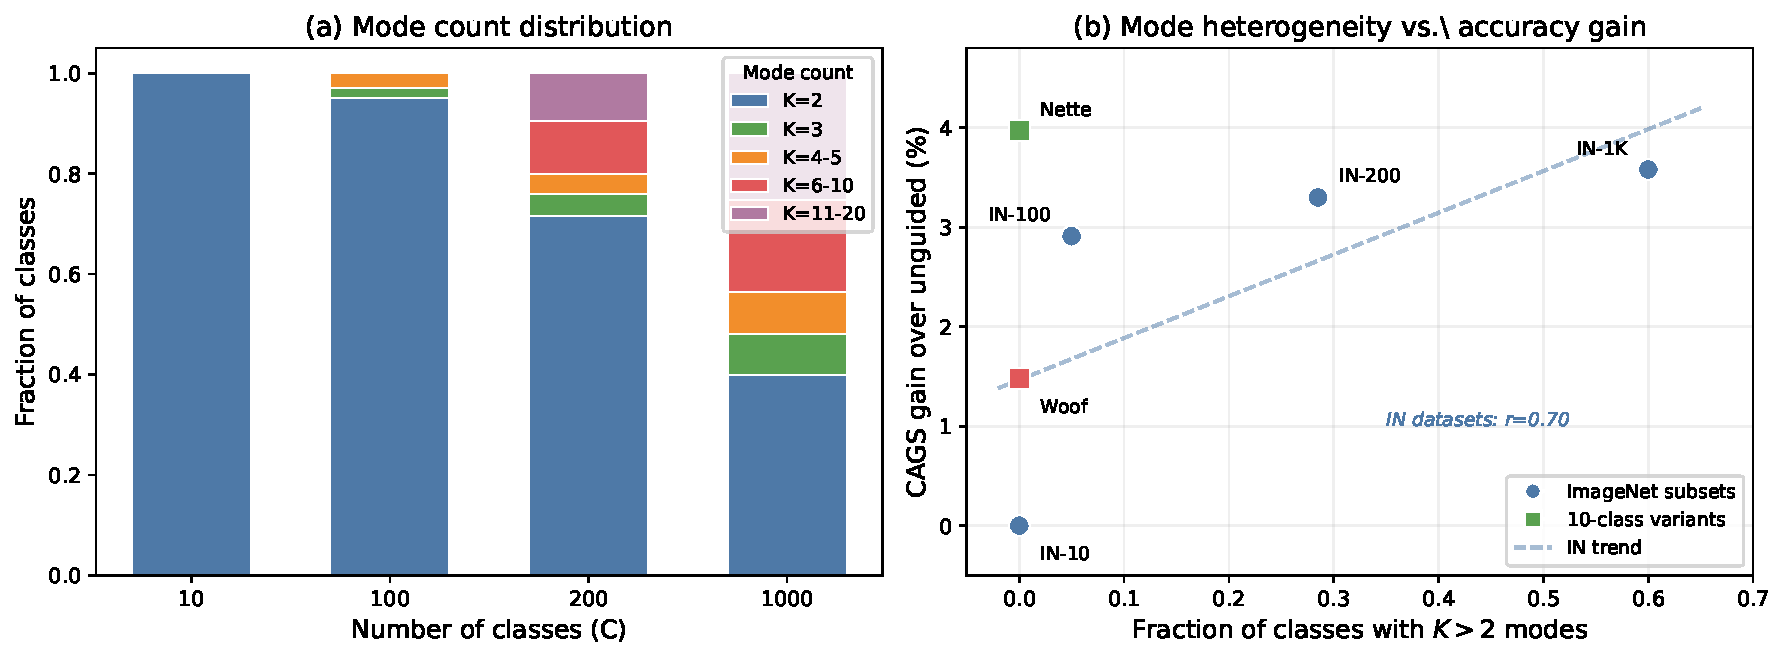
\includegraphics[width=\columnwidth]{figures/theorem1_fit.pdf}
\caption{Quantitative validation of Theorem~\ref{thm:adaptivity-gap}. (a)~Distribution of mode counts ($K$) across ImageNet subsets with increasing class count. The fraction of classes with $K > 2$ grows from $0\%$ ($C{=}10$) to $60\%$ ($C{=}1000$), reflecting increasing mode structure heterogeneity. (b)~Mode heterogeneity (fraction of classes with $K > 2$) vs.\ actual CAGS accuracy gain. ImageNet subsets (circles) show a positive trend; 10-class variants (squares) demonstrate that class composition matters even at fixed $C$.}
\label{fig:theorem1-fit}
\end{figure}

\paragraph{Why TAGS fails: temporal variation cannot substitute for class variation.}
\tags{} replaces the constant $\lambda$ with a time-varying schedule $\lambda(t)$, varying guidance across timesteps but applying the same $\lambda(t)$ to all classes at each $t$. The adaptivity gap at timestep $t$ is:
\begin{equation}
\Delta(t) = \frac{1}{C}\sum_{c=1}^C \frac{\beta\,\sigma_c^2}{2}\,(\lambda_c^* - \lambda(t))^2.
\end{equation}
The optimal per-class guidance $\lambda_c^* = v_c / (\beta\,\sigma_c^2)$ (Proposition~\ref{prop:opt-lambda}) depends on intra-class properties ($v_c, \boldsymbol{\pi}_c$) and is independent of the timestep $t$, because the mode structure is a property of the class-conditional distribution, not the noise level. Therefore, the best temporal schedule $\lambda(t)$ at each $t$ is the cross-class average $\bar{\lambda} = \frac{1}{C}\sum_c \lambda_c^*$, yielding $\Delta_{\text{TAGS}} = \sum_t \Delta(t) = T \cdot \Delta_{\text{fixed}}$, where $T$ is the number of timesteps. This is exactly $T$ times the fixed-guidance adaptivity gap---TAGS provides \emph{no reduction} in the adaptivity gap because it varies $\lambda$ along a dimension (time) where the optimal $\lambda_c^*$ is constant, while failing to vary it along the dimension (class) where $\lambda_c^*$ actually differs. In contrast, \cags{} varies $\lambda$ across classes, directly targeting the source of suboptimality.

\paragraph{Why IAST fails: range compression reduces the adaptivity gap.}
\iast{} scales the guidance range $[\lambda_{\min}, \lambda_{\max}]$ by a factor $s(\text{IPC}) = \min(1, \log(\text{IPC}+1)/\log(\text{IPC}_{\text{ref}}+1))$, compressing the range when $\text{IPC} < \text{IPC}_{\text{ref}} = 10$. The effective per-class guidance becomes $s \cdot \lambda_c$, and the adaptivity gap scales as:
\begin{equation}
\Delta_{\text{IAST}} = \frac{1}{C}\sum_c \frac{\beta\,\sigma_c^2}{2}\,(\lambda_c^* - s\,\lambda_c)^2 \approx s^2 \cdot \Delta_{\text{CAGS}},
\end{equation}
where the approximation holds when $s \cdot \lambda_c$ is close to $s \cdot \bar{\lambda}$ (i.e., the compressed guidance is nearly uniform). At IPC=1, $s \approx 0.29$, so $\Delta_{\text{IAST}} \approx 0.084 \cdot \Delta_{\text{CAGS}}$---a $92\%$ reduction in the adaptivity gap. Rather than protecting against over-sharpening, IAST eliminates the per-class differentiation that drives CAGS's benefit. At IPC $\geq 10$, $s = 1$ and IAST is transparent, which is consistent with our experimental finding that IAST is neutral at IPC=10 but harmful at IPC=1. This analysis reveals that the IPC dimension, like the temporal dimension, is not the axis along which adaptive guidance provides value---the class axis is.

\paragraph{Remark on assumptions.}
The well-separated modes assumption (Lemma~\ref{lem:cfg-modes}) is an idealization; in practice, modes may overlap and the $p(\mathbf{x})^{-\lambda}$ term introduces inter-class effects. However, the qualitative predictions---that optimal $\lambda$ increases with $v_c$ and $H_c$, that separability is irrelevant, and that the adaptivity gap grows with class heterogeneity---are robust to relaxation of this assumption, as confirmed by experiments across datasets, architectures, and scales (Sections~\ref{sec:experiments}--\ref{sec:dd-baselines}).
